%%% Question %%%
\section{Scheme Lists}
\begin{blocksection}
\begin{nonsol}
Scheme has linked lists built in. You can make the following analogy:
\begin{center}
\begin{tabular}{ |l|l| }
\hline
 \texttt{Link(1, Link.empty)} & \texttt{(cons 1 nil)} \\
 \texttt{a = Link(1, Link(2, Link.empty))} & \texttt{(define a (cons 1 (cons 2 nil)))}  \\
 \texttt{a.first} & \texttt{(car a)} \\
 \texttt{a.rest} & \texttt{(cdr a)} \\
 \hline
\end{tabular}

\end{center}
However, \textbf{Scheme \texttt{cons} is more powerful}, as it allows its second argument to not be a list. Try the following out in the interpreter. Draw box and pointers when appropriate. Ask your mentor if you're unsure what's going on. You aren't expected to understand this completely on your own.
\question What will Scheme output? Draw box-and-pointer diagrams to help determine this.
\end{nonsol}

\begin{lstlisting}
scm> (cons 1 2)
\end{lstlisting}
\begin{solution}[0.25in]
\texttt{(1 . 2)}
\begin{center}
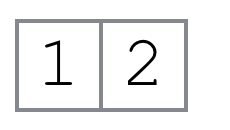
\includegraphics[scale=1]{scheme_lists_1}
\end{center}
\end{solution}

\begin{lstlisting}
scm> (cons 1 (cons 2 nil))
\end{lstlisting}
\begin{solution}[0.25in]
\texttt{(1 2)}
\begin{center}
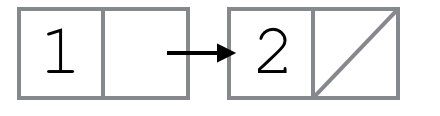
\includegraphics[scale=0.7]{scheme_lists_2}
\end{center}
\end{solution}

\begin{lstlisting}
scm> (cons 1 '(2 3 4 5))
\end{lstlisting}
\begin{solution}[0.25in]
\texttt{(1 2 3 4 5)}
\begin{center}
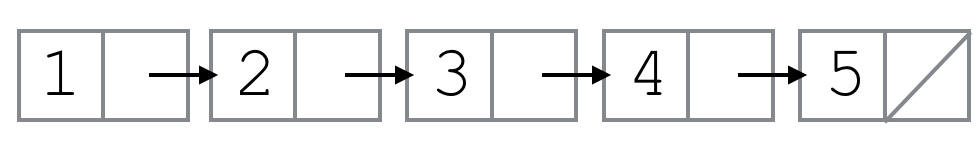
\includegraphics[scale=0.7]{scheme_lists_3}
\end{center}
\end{solution}

\begin{lstlisting}
scm> (cons 1 '(2 (cons 3 4))
\end{lstlisting}
\begin{solution}[0.25in]
\texttt{(1 2 (cons 3 4))}
\begin{center}
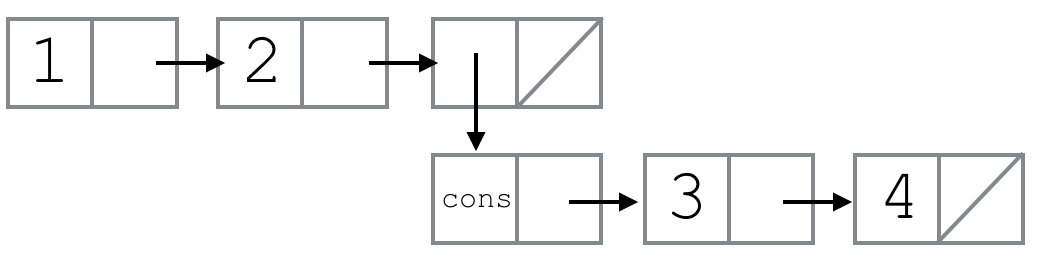
\includegraphics[scale=0.7]{scheme_lists_4}
\end{center}
\end{solution}

\begin{lstlisting}
scm> (cons 1 (2 (cons 3 4)))
\end{lstlisting}
\begin{solution}[.25in]
\begin{lstlisting}
eval: bad function in : (2 (cons 3 4))
\end{lstlisting}
\end{solution}
\end{blocksection}

\begin{blocksection}
\begin{lstlisting}
scm> (define a '(1 2 . 3))
\end{lstlisting}
\begin{solution}[.25in]
\begin{lstlisting}
a
\end{lstlisting}
\end{solution}

\begin{lstlisting}
scm> a
\end{lstlisting}
\begin{solution}[.25in]
\begin{lstlisting}
(1 2 . 3)
\end{lstlisting}
\end{solution}

\begin{lstlisting}
scm> (car a)
\end{lstlisting}
\begin{solution}[.25in]
\begin{lstlisting}
1
\end{lstlisting}
\end{solution}

\begin{lstlisting}
scm> (cdr a)
\end{lstlisting}
\begin{solution}[.25in]
\begin{lstlisting}
(2 . 3)
\end{lstlisting}
\end{solution}

\begin{lstlisting}
scm> (cadr a)
\end{lstlisting}
\begin{solution}[.25in]
\begin{lstlisting}
2
\end{lstlisting}
\end{solution}

How can we get the 3 out of a?
\begin{solution}[.25in]
\begin{lstlisting}
(cddr a)
\end{lstlisting}
\end{solution}
\end{blocksection}